%% Appendices: placed directly after the Conclusion and before the declarations and references.
\appendix
\renewcommand{\thetable}{\thesection.\arabic{table}}
\renewcommand{\thefigure}{\thesection.\arabic{figure}}
\renewcommand{\theequation}{\thesection.\arabic{equation}}

% an unnumbered heading, so a reader can see where the appendices begin
\section*{Appendices}

\section{The question schema}
\label{app:schema}
\setcounter{table}{0}\setcounter{figure}{0}\setcounter{equation}{0}

Table~\ref{tab:schema-full} reproduces every question in the schema as it was sent to the
model, with its type, its gate where it has one, and the complete instruction and criteria
text. The text is the entire specification of each variable, because the model sees nothing
else, and the human coders of Section~\ref{sec:reference} and the frontier models of
Section~\ref{sec:res-frontier} received the same text verbatim. The schema was produced in two steps that the released files record. A first version was written from the design rules of Section~\ref{sec:schema} and
run on a development sample of \SchemaValidateCompared{} narratives, and the error analysis of
that run produced the exclusion clause of the aggression question, whose effect is reported
in Section~\ref{sec:schema}. The file reproduced here is the second version, which is the one
used for the second-stage run, the reference set and the frontier arms, and it is released
with the code together with the lean first-stage schema of \NLeanQuestions{} presence
questions. Instructions refer to the narrative by its key in the state object, and criteria
for a presence question name the boundary cases that count and do not count, which is where
most of the design effort went. The residual-identifier question is included in the file
because it ships with the schema, but it was run as a separate display screen and was not part
of the population coding.

\begin{small}\rmfamily
\setlength{\tabcolsep}{3.0pt}
\begin{longtable}{lrr>{\raggedright\arraybackslash}p{267.2pt}}
\caption{The full question schema, version 1.1, as sent to the model.}\label{tab:schema-full}\\
\toprule
\jevhead{id} & \jevhead{type} & \jevhead{gate} & \jevheadp{instruction and criteria} \\
\midrule
\endfirsthead
\multicolumn{4}{@{}l}{\rmfamily\small\textit{Table \ref{tab:schema-full}, continued}}\\
\toprule
\jevhead{id} & \jevhead{type} & \jevhead{gate} & \jevheadp{instruction and criteria} \\
\midrule
\endhead
\bottomrule
\multicolumn{4}{@{}r}{\rmfamily\small\textit{continued on the next page}}\\
\endfoot
\bottomrule
\multicolumn{4}{@{}p{\linewidth}@{}}{\rmfamily\small\vspace{2pt}\textit{Note:}~Text is reproduced from \texttt{schemas/crash\_factors\_v1\_1.json} without abbreviation. A gated question is interpreted only when its gate exceeds $\tau_g = 0.5$, otherwise it takes its no-match option. \texttt{pii\_residual} ships in the same file but was run separately as the display screen, outside the Stage 1 and Stage 2 calls.}\\
\endlastfoot
\texttt{preg\_mentioned} & noul & -- & The 'narrative' states that a person involved in the crash was pregnant. \newline \textit{true}: Any explicit statement that a driver, passenger, pedestrian, or other involved person is pregnant, e.g. 'was 6 months pregnant', 'pregnant driver', 'expecting'. \newline \textit{false}: No pregnancy is stated. Mentions of children, infants, or car seats do not count. \\
\texttt{medical\_episode} & noul & -- & The 'narrative' states that a driver experienced a medical event (seizure, fainting, blackout, diabetic episode, heart attack, stroke, or similar) before or during the crash. \newline \textit{true}: A medical event of the driver is described as occurring before or during the crash, whether confirmed or suspected by the officer. \newline \textit{false}: No medical event of the driver is described. Injuries caused by the crash, or transport to a hospital for crash injuries, do not count. \\
\texttt{drug\_involved} & noul & -- & The 'narrative' states or suspects that a driver was under the influence of drugs or medication (not alcohol). \newline \textit{true}: Any statement that a driver used, was impaired by, or was suspected of using illegal drugs, marijuana, prescription medication, or other substances other than alcohol. \newline \textit{false}: No drug or medication involvement of a driver is mentioned. Alcohol-only impairment does not count. \\
\texttt{alcohol\_involved} & noul & -- & The 'narrative' states or suspects that a driver had been drinking alcohol or was intoxicated by alcohol. \newline \textit{true}: Any statement that a driver had been drinking, smelled of alcohol, was DWI or DUI, or was suspected of alcohol intoxication. \newline \textit{false}: No alcohol involvement of a driver is mentioned. \\
\texttt{hydroplane} & noul & -- & The 'narrative' states that a vehicle hydroplaned or lost traction because of water on the roadway. \newline \textit{true}: The word hydroplane appears, or the narrative says a vehicle lost traction, skidded, or lost control because of rain, wet roadway, or standing water. \newline \textit{false}: No loss of traction due to water is described. Wet conditions mentioned without loss of control do not count. \\
\texttt{vehicle\_defect} & noul & -- & The 'narrative' states that a mechanical failure of a vehicle (tire blowout, brake failure, steering failure, or similar) contributed to the crash. \newline \textit{true}: A tire blowout, tread separation, brake failure, steering failure, stuck accelerator, or other mechanical defect is described as contributing to the crash. \newline \textit{false}: No mechanical failure is described. Damage caused by the crash does not count. \\
\texttt{fatigue} & noul & -- & The 'narrative' states that a driver fell asleep, dozed off, was drowsy, or was fatigued. \newline \textit{true}: A driver is described as asleep, falling asleep, nodding off, drowsy, tired, or fatigued before the crash. \newline \textit{false}: No sleep or fatigue of a driver is mentioned. \\
\texttt{aggression} & noul & -- & The 'narrative' describes road rage, aggressive driving directed at another road user, or a physical or verbal confrontation between people involved. \newline \textit{true}: Road rage, brake-checking, chasing, threatening, arguing, fighting, or a confrontation before or after the crash is described. \newline \textit{false}: No aggression or confrontation is described. Ordinary traffic violations without hostility do not count. A police pursuit, a traffic stop, an officer chasing or stopping a vehicle, and a driver evading or fleeing from police do not count. A driver leaving the scene of the crash does not count by itself. \\
\texttt{intentional} & noul & -- & The 'narrative' states or suspects that a vehicle was used intentionally to cause the crash (assault with a vehicle, deliberate ramming, or a suicide attempt). \newline \textit{true}: The crash is described as deliberate, intentional, on purpose, an assault with a vehicle, or a suicide attempt. \newline \textit{false}: The crash is described as unintentional, or intent is not mentioned. \\
\texttt{hit\_and\_run} & noul & -- & The 'narrative' states that a driver left the scene of the crash without stopping to provide information. \newline \textit{true}: A driver fled, left the scene, failed to stop and render aid, or drove away without exchanging information. \newline \textit{false}: All drivers remained at the scene, or leaving the scene is not mentioned. \\
\texttt{animal\_involved} & noul & -- & The 'narrative' states that an animal on or near the roadway was involved in the crash or in the driver's evasive action. \newline \textit{true}: A vehicle struck an animal, or swerved or braked to avoid an animal. \newline \textit{false}: No animal is mentioned as involved. \\
\texttt{wrong\_way} & noul & -- & The 'narrative' states that a vehicle was traveling the wrong way on a roadway, ramp, or lane designated for the opposite direction. \newline \textit{true}: A vehicle is described as going the wrong way, wrong direction, or against traffic on a one-way road, divided highway, or ramp. \newline \textit{false}: No wrong-way travel is described. Crossing the center line during a loss of control does not count. \\
\texttt{phone\_use} & noul & -- & The 'narrative' states that a driver was using a phone or mobile device at the time of the crash. \newline \textit{true}: A driver is described as texting, talking on a phone, looking at a phone, or using a mobile device. \newline \textit{false}: No phone or device use is mentioned. General 'distracted' or 'inattention' without a device does not count. \\
\texttt{unbelted} & noul & -- & The 'narrative' states that a vehicle occupant was not wearing a seat belt. \newline \textit{true}: An occupant is described as unrestrained, not wearing a seat belt, or unbelted. \newline \textit{false}: Seat belt use is not mentioned, or occupants are described as belted. \\
\texttt{transported} & noul & -- & The 'narrative' states that a person was transported to a hospital or medical facility. \newline \textit{true}: A person was transported by EMS, ambulance, helicopter, or private vehicle to a hospital, medical center, or clinic. \newline \textit{false}: No transport to a medical facility is mentioned, or people refused transport. \\
\texttt{witness\_cited} & noul & -- & The 'narrative' cites a statement from a witness who was not a driver or occupant of the involved vehicles. \newline \textit{true}: A witness, bystander, or independent observer's statement is described. \newline \textit{false}: Only driver, passenger, or officer statements appear, or no statements appear. \\
\texttt{medical\_type} & choice & \texttt{medical\_episode} & Which type of driver medical event does the 'narrative' describe as occurring before or during the crash? \newline \textit{seizure}: Seizure or epileptic episode. \newline \textit{loss\_of\_consciousness}: Fainting, passing out, blacking out, syncope, or becoming unresponsive without a stated cause. \newline \textit{diabetic}: Diabetic episode, low blood sugar, hypoglycemia, or insulin-related event. \newline \textit{cardiac}: Heart attack, cardiac arrest, chest pain, or other heart event. \newline \textit{stroke}: Stroke or stroke-like symptoms. \newline \textit{other\_medical}: Another medical condition or episode of the driver, such as dementia, dizziness, or an unspecified medical emergency. \newline \textit{none}: No driver medical event is described. \\
\texttt{drug\_class} & choice & \texttt{drug\_involved} & Which category of drug or medication does the 'narrative' associate with a driver? Choose based only on what the narrative names. \newline \textit{marijuana}: Marijuana, THC, cannabis, or weed. \newline \textit{stimulant}: Methamphetamine, cocaine, amphetamines, or other stimulants. \newline \textit{opioid}: Heroin, fentanyl, oxycodone, hydrocodone, or other opioids. \newline \textit{sedative\_prescription}: Xanax, benzodiazepines, sleeping pills, muscle relaxers, or other prescription sedatives. \newline \textit{unspecified\_drug}: Drugs, narcotics, a controlled substance, or medication mentioned without naming the type. \newline \textit{none}: No drug or medication is mentioned. \\
\texttt{preg\_role} & choice & \texttt{preg\_mentioned} & What was the role of the pregnant person in the crash according to the 'narrative'? \newline \textit{driver}: The pregnant person was driving one of the vehicles. \newline \textit{passenger}: The pregnant person was a passenger in one of the vehicles. \newline \textit{pedestrian\_or\_other}: The pregnant person was a pedestrian, cyclist, or otherwise not inside a vehicle. \newline \textit{no\_pregnancy}: The narrative does not state that anyone was pregnant. \\
\texttt{preg\_outcome} & choice & \texttt{preg\_mentioned} & What does the 'narrative' state about the condition of the pregnant person after the crash? \newline \textit{no\_complaint}: The pregnant person reported no injury or the narrative gives no complaint. \newline \textit{pain\_or\_evaluation}: The pregnant person complained of pain, tightness, or discomfort, or was checked by EMS but not transported. \newline \textit{transported}: The pregnant person was transported to a hospital or medical facility as a precaution or for injury. \newline \textit{fetal\_harm}: The narrative states harm to, or loss of, the unborn child. \newline \textit{no\_pregnancy}: The narrative does not state that anyone was pregnant. \\
\texttt{preg\_stage} & choice & \texttt{preg\_mentioned} & What stage of pregnancy does the 'narrative' state for the pregnant person? \newline \textit{early}: Up to 13 weeks, or 1 to 3 months pregnant, or described as first trimester or early pregnancy. \newline \textit{mid}: 14 to 27 weeks, or 4 to 6 months pregnant, or described as second trimester. \newline \textit{late}: 28 weeks or more, or 7 to 9 months pregnant, or described as third trimester, due soon, or full term. \newline \textit{stage\_not\_stated}: Pregnancy is stated but no weeks, months, or trimester is given. \newline \textit{no\_pregnancy}: The narrative does not state that anyone was pregnant. \\
\texttt{animal\_type} & choice & \texttt{animal\_involved} & Which kind of animal does the 'narrative' describe as involved in the crash? \newline \textit{deer}: Deer. \newline \textit{dog}: Dog. \newline \textit{livestock}: Cow, cattle, horse, goat, or other livestock. \newline \textit{feral\_hog}: Hog, feral hog, wild boar, or pig. \newline \textit{other\_animal}: Any other animal, such as coyote, cat, or an unnamed animal. \newline \textit{none}: No animal is described as involved. \\
\texttt{defect\_type} & choice & \texttt{vehicle\_defect} & Which kind of vehicle mechanical failure does the 'narrative' describe as contributing to the crash? \newline \textit{tire}: Tire blowout, flat tire, or tread separation. \newline \textit{brakes}: Brake failure or brakes not working. \newline \textit{steering\_or\_suspension}: Steering failure, wheel came off, axle or suspension failure. \newline \textit{other\_mechanical}: Another mechanical failure such as engine stall, stuck accelerator, or trailer hitch failure. \newline \textit{none}: No mechanical failure is described. \\
\texttt{surface\_narr} & choice & -- & What roadway surface condition does the 'narrative' state at the time of the crash? \newline \textit{dry}: The roadway is described as dry. \newline \textit{wet}: The roadway is described as wet, rainy, or having standing water. \newline \textit{ice\_or\_snow}: The roadway is described as icy, frozen, slick from ice, or snowy. \newline \textit{other\_surface}: Another surface hazard is described, such as gravel, oil, mud, sand, or debris. \newline \textit{not\_stated}: The narrative does not describe the surface condition. \\
\texttt{narrative\_detail} & score & -- & How much crash-relevant detail does the 'narrative' contain? \newline \textit{level 0}: Boilerplate or a single sentence with no description of how the crash happened. \newline \textit{level 1}: A basic sequence of vehicle movements and the collision, without statements or contributing factors. \newline \textit{level 2}: A detailed account including driver or witness statements, contributing factors, or officer findings. \\
\texttt{emotion\_intensity} & score & -- & How intense is the emotional state of any driver described in the 'narrative' before or after the crash? \newline \textit{level 0}: No emotional state is described. \newline \textit{level 1}: A driver is described as upset, frustrated, crying, shaken, or scared. \newline \textit{level 2}: A driver is described as angry, hostile, yelling, threatening, or violent. \\
\texttt{injury\_narr} & score & -- & What is the most severe injury outcome stated in the 'narrative' for any person? \newline \textit{level 0}: No injury is mentioned, or the narrative says no one was injured. \newline \textit{level 1}: A person complained of pain or possible injury but was not transported. \newline \textit{level 2}: A person had a visible injury or was transported to a hospital. \newline \textit{level 3}: A person was pronounced dead or the narrative describes a fatality. \\
\texttt{pii\_residual} & noul & -- & The 'narrative' contains a person's full name, date of birth, driver license or ID number, home address, or phone number that is not already replaced by a placeholder. \newline \textit{true}: An actual name, date of birth, license or ID number, street address, or phone number appears as literal text. \newline \textit{false}: No such identifier appears, or every identifier has been replaced by a placeholder such as [NAME] or [PHONE]. \\
\end{longtable}
\end{small}


\section{Keyword families and the coded-field mapping}
\label{app:keywords}
\setcounter{table}{0}\setcounter{figure}{0}\setcounter{equation}{0}

The rule baseline of Section~\ref{sec:reference} is a set of case-insensitive regular
expressions, one family per variable, and Table~\ref{tab:keywords} lists them as they appear
in the scripts that apply them. The first ten families were written to over-find rather than
to be precise, because their original purpose was to enrich the rare classes of the
second-stage frame and to provide a population keyword rate over all \Ncorpus{} narratives.
They were tuned only on the development sample and never on any evaluated narrative. The
last three families, for alcohol involvement, phone use and restraint use, were added so that
the baseline covers every variable that has a coded reference, since comparing a
macro-averaged score over different variable sets would not be a comparison. Those three
were scored on the working set of narratives only. The residual-identifier patterns of
Section~\ref{sec:corpus} are of the same kind and are listed in the released code beside
them. Table~\ref{tab:coded-map} gives the mapping from each narrative variable to the coded
CRIS fields that define its reference, which is implemented in the released join script over
the crash-unit-person extract. Each reference is true for a crash when the rule holds on any
person or unit row of that crash, because a contributing factor is recorded per unit and a
restraint or test result per person. The hydroplaning reference is a proxy built from the
loss-of-control, surface and weather codes, because CRIS has no hydroplaning field. The
final row is the opposite-direction collision type that the original plan proposed for
wrong-way travel, retained only as a sensitivity check after it proved a factor of
\WrongWayProxyRatio{} too broad.

\begin{small}\rmfamily
\setlength{\tabcolsep}{3.0pt}
\begin{longtable}{l>{\raggedright\arraybackslash}p{71.2pt}>{\raggedright\arraybackslash}p{44.5pt}>{\raggedright\arraybackslash}p{289.2pt}}
\caption{Regular-expression families of the rule baseline.}\label{tab:keywords}\\
\toprule
\jevhead{family} & \jevheadp{narrative variable} & \jevheadp{scope} & \jevheadp{regular expression (case-insensitive)} \\
\midrule
\endfirsthead
\multicolumn{4}{@{}l}{\rmfamily\small\textit{Table \ref{tab:keywords}, continued}}\\
\toprule
\jevhead{family} & \jevheadp{narrative variable} & \jevheadp{scope} & \jevheadp{regular expression (case-insensitive)} \\
\midrule
\endhead
\bottomrule
\multicolumn{4}{@{}r}{\rmfamily\small\textit{continued on the next page}}\\
\endfoot
\bottomrule
\multicolumn{4}{@{}p{\linewidth}@{}}{\rmfamily\small\vspace{2pt}\textit{Note:}~The first ten families apply to all narratives and provide the population keyword rates of Table~\ref{tab:prevalence}. The last three were added so the baseline covers every variable with a coded reference, and were scored on the working set only. Patterns are read from the scripts that apply them.}\\
\endlastfoot
preg & preg\_mentioned & all narratives & \texttt{pregnan|\allowbreak{}unborn|\allowbreak{}fetus|\allowbreak{}fetal|\allowbreak{}trimester|\allowbreak{}weeks along|\allowbreak{}miscarr} \\
medical & medical\_episode & all narratives & \texttt{seizure|\allowbreak{}diabet|\allowbreak{}passed out|\allowbreak{}blacked out|\allowbreak{}fainted|\allowbreak{}heart attack|\allowbreak{}stroke|\allowbreak{}unconscious|\allowbreak{}medical (episode|\allowbreak{}condition|\allowbreak{}emergency|\allowbreak{}event)|\allowbreak{}dementia|\allowbreak{}alzheimer} \\
drug & drug\_involved & all narratives & \texttt{marijuana|\allowbreak{}methamphetamine|\allowbreak{}meth |\allowbreak{}cocaine|\allowbreak{}fentanyl|\allowbreak{}xanax|\allowbreak{}heroin|\allowbreak{}pills|\allowbreak{}narcotic|\allowbreak{}controlled substance|\allowbreak{}under the influence of (a )?drug} \\
hydro & hydroplane & all narratives & \texttt{hydroplan} \\
defect & vehicle\_defect & all narratives & \texttt{tire blow|\allowbreak{}blowout|\allowbreak{}blew out|\allowbreak{}brake fail|\allowbreak{}brakes fail|\allowbreak{}mechanical fail|\allowbreak{}steering fail} \\
rage & aggression & all narratives & \texttt{road rage|\allowbreak{}angry|\allowbreak{}anger|\allowbreak{}enraged|\allowbreak{}argument|\allowbreak{}fight|\allowbreak{}confront|\allowbreak{}brandish|\allowbreak{}assault} \\
fatigue & fatigue & all narratives & \texttt{fell asleep|\allowbreak{}asleep|\allowbreak{}drowsy|\allowbreak{}fatigue|\allowbreak{}nodded off} \\
intent & intentional & all narratives & \texttt{suicid|\allowbreak{}intentional|\allowbreak{}deliberate|\allowbreak{}on purpose|\allowbreak{}rammed} \\
wrongway & wrong\_way & all narratives & \texttt{wrong way|\allowbreak{}wrong direction} \\
animal & animal\_involved & all narratives & \texttt{deer|\allowbreak{}hog|\allowbreak{}cow|\allowbreak{}horse|\allowbreak{}dog|\allowbreak{}coyote|\allowbreak{}cattle} \\
alcohol & alcohol\_involved & working set & \texttt{\textbackslash{}balcohol|\allowbreak{}intoxicat|\allowbreak{}\textbackslash{}bdwi\textbackslash{}b|\allowbreak{}\textbackslash{}bdui\textbackslash{}b|\allowbreak{}drunk|\allowbreak{}\textbackslash{}bbac\textbackslash{}b|\allowbreak{}been drinking|\allowbreak{}odor of an alcoholic|\allowbreak{}open container|\allowbreak{}breathalyz|\allowbreak{}field sobriety} \\
phone & phone\_use & working set & \texttt{cell ?phone|\allowbreak{}cellular|\allowbreak{}mobile (phone|\allowbreak{}device)|\allowbreak{}texting|\allowbreak{}\textbackslash{}btext(ed|\allowbreak{}ing)?\textbackslash{}b|\allowbreak{}on (the|\allowbreak{}his|\allowbreak{}her|\allowbreak{}their) phone|\allowbreak{}looking at (his|\allowbreak{}her|\allowbreak{}their) phone} \\
unbelted & unbelted & working set & \texttt{not wearing (a )?(seat ?belt|\allowbreak{}safety belt)|\allowbreak{}unbelted|\allowbreak{}unrestrained|\allowbreak{}no (seat ?belt|\allowbreak{}restraint)|\allowbreak{}seat ?belt was not|\allowbreak{}without a seat ?belt} \\
\end{longtable}
\end{small}

\begin{small}\rmfamily
\setlength{\tabcolsep}{3.0pt}
\begin{longtable}{>{\raggedright\arraybackslash}p{73.0pt}r>{\raggedright\arraybackslash}p{203.7pt}>{\raggedright\arraybackslash}p{70.6pt}}
\caption{Mapping from narrative variables to coded CRIS reference fields.}\label{tab:coded-map}\\
\toprule
\jevheadp{narrative variable} & \jevhead{reference column} & \jevheadp{CRIS fields and values} & \jevheadp{aggregation to crash level} \\
\midrule
\endfirsthead
\multicolumn{4}{@{}l}{\rmfamily\small\textit{Table \ref{tab:coded-map}, continued}}\\
\toprule
\jevheadp{narrative variable} & \jevhead{reference column} & \jevheadp{CRIS fields and values} & \jevheadp{aggregation to crash level} \\
\midrule
\endhead
\bottomrule
\multicolumn{4}{@{}r}{\rmfamily\small\textit{continued on the next page}}\\
\endfoot
\bottomrule
\multicolumn{4}{@{}p{\linewidth}@{}}{\rmfamily\small\vspace{2pt}\textit{Note:}~Each reference is true for a crash when the rule holds on any of its person or unit rows. The hydroplaning reference is a proxy built from surface, weather and loss-of-control codes, because CRIS has no hydroplaning field. The final row is the opposite-direction collision type the original plan proposed for wrong-way travel, retained only as a sensitivity check.}\\
\endlastfoot
alcohol\_involved & \texttt{coded\_alcohol} & \texttt{Contrib\_Factr\_1\_ID} or \texttt{Contrib\_Factr\_2\_ID} matches ``Under Influence - Alcohol'' or ``Had Been Drinking''; or \texttt{Prsn\_Alc\_Rslt\_ID} = 1; or \texttt{Prsn\_Bac\_Test\_Rslt} $>$ 0 & any person or unit row of the crash \\
drug\_involved & \texttt{coded\_drug} & contributing factor matches ``Under Influence - Drug''; or \texttt{Prsn\_Drg\_Rslt\_ID} = 1 & any row \\
fatigue & \texttt{coded\_fatigue} & contributing factor matches ``Fatigued Or Asleep'' & any row \\
medical\_episode & \texttt{coded\_medical} & contributing factor matches ``Ill (Explain In Narrative)'' & any row \\
animal\_involved & \texttt{coded\_animal} & contributing factor matches ``Animal On Road''; or \texttt{Harm\_Evnt\_ID} contains ``Animal'' & any row \\
phone\_use & \texttt{coded\_phone} & contributing factor matches ``Cell/Mobile Device Use'' & any row \\
unbelted & \texttt{coded\_unbelted} & \texttt{Prsn\_Rest\_ID} equals ``None'' (the only unbelted code; ``Not Applicable'' excluded) & any person row \\
hydroplane & \texttt{coded\_hydro\_proxy} & \texttt{Othr\_Factr\_ID} contains ``Lost Control Or Skidded'' and (\texttt{Surf\_Cond\_ID} contains ``Wet'' or ``Standing Water'', or \texttt{Wthr\_Cond\_ID} contains ``Rain'') & any row; proxy reference \\
wrong\_way & \texttt{coded\_wrongway} & contributing factor matches ``Wrong Way - One Way Road'', ``Wrong Side - Not Passing'' or ``Wrong Side - Approach'' & any row \\
(sensitivity only) & \texttt{coded\_wrongway\_proxy} & \texttt{FHE\_Collsn\_ID} contains ``Opposite Direction'' & any row; not used as a reference \\
\end{longtable}
\end{small}


\section{Coder protocol and additional reliability diagrams}
\label{app:coders}
\setcounter{table}{0}\setcounter{figure}{0}\setcounter{equation}{0}

The human reference set of Section~\ref{sec:reference} was produced under a written protocol
that this appendix summarizes, and Figures~\ref{fig:goldrel} and \ref{fig:goldprec} draw the
two human-referenced diagrams that the main text refers to. The protocol defined the task as
one narrow question repeated, whether the narrative states the factor, under the governing
rule to label what the narrative states rather than what probably happened. A crash that an
experienced analyst would read as alcohol-involved is therefore labeled negative if the
officer did not write it down. That rule inverts the usual assumption that more domain
expertise is better, because the dominant risk is over-inference. Coders who know crashes
may fill in what the officer omitted, agree with each other, and produce a reference that is
confidently wrong in the direction the model might also be wrong. The panel was therefore
mixed by design, with one crash-data practitioner who reads officer shorthand, one
transportation-safety researcher familiar with the constructs, and one careful non-specialist
reader who cannot over-infer and who serves as the check on the other two. Coders were
required to be independent of the modeling work, never to have seen the model's outputs or
helped write the criteria, and not to discuss items while coding. All three first coded a
shared calibration block, which was reviewed together once to catch inference, ambiguous
criteria and shorthand the non-specialist could not read, after which no further discussion
took place. Each coder then labeled an allocation of narratives determined by position in a
fixed roster, with every narrative coded by two of the three and the calibration block by all
three. The roster rule was deterministic and fixed before any narrative was seen. Narratives
were held in the order the export produced, and the calibration block occupied the first
positions and was assigned to every coder. Each later position went to the two coders whose
index matched that position under a fixed rotation, so no coder chose a narrative and no
narrative was reassigned after labeling began. Each judgment carried the coder identifier, the
time taken and a yes, no or unclear verdict. Reliability was computed from the double- and
triple-coded pairs as reported in Section~\ref{sec:reference}, majority labels were formed, and
ties and unclear verdicts were recorded as disputed and excluded.

The calibration weights of Section~\ref{sec:reference} are built from the frame rather than
from the labels, and their construction is recorded here in full. The population is the
second-stage random stratum. For each of the \FrontierNVars{} presence variables the population
is divided into the cells \GoldBinsText{} and the labeled pairs falling in each cell are scaled
so that their weights sum to the population count of that cell. \DesignNActivePairs{} of the
pairs entered through the active route, with assignment probability one, and
\DesignNControlPairs{} through the control route, with assignment probability
\GoldNegControls{} divided by the narrative's count of low-probability variables. Cells holding
fewer than \DesignMinCell{} labeled pairs were merged with an adjacent cell of the same
variable before the scaling, which affected \DesignNCollapsed{} variables, and the merges are
listed in the released design report. The weights span a factor of \DesignWeightRatio{} and
give a design effect of \DesignDeff{}, with per-variable effective sample sizes running from
\DesignNEffVarLo{} to \DesignNEffVarHi{}. The cluster bootstrap resamples narratives within the
\DesignNStrata{} draw routes the frame records, which are the cells the greedy rule drew each
narrative to fill.

\begin{small}\rmfamily
\setlength{\tabcolsep}{4.0pt}
\begin{longtable}{l>{\raggedright\arraybackslash}p{186.9pt}rrrr}
\caption{Unresolved pairs and the sensitivity of the headline results to them.}\label{tab:exclusions}\\
\toprule
\jevhead{block} & \jevheadp{item} & \jevhead{count} & \jevhead{$F_1$} & \jevhead{ECE} & \jevhead{$H(0.90)$ \%} \\
\midrule
\endfirsthead
\multicolumn{6}{@{}l}{\rmfamily\small\textit{Table \ref{tab:exclusions}, continued}}\\
\toprule
\jevhead{block} & \jevheadp{item} & \jevhead{count} & \jevhead{$F_1$} & \jevhead{ECE} & \jevhead{$H(0.90)$ \%} \\
\midrule
\endhead
\bottomrule
\multicolumn{6}{@{}r}{\rmfamily\small\textit{continued on the next page}}\\
\endfoot
\bottomrule
\multicolumn{6}{@{}p{\linewidth}@{}}{\rmfamily\small\vspace{2pt}\textit{Note:}~The \ExclN{} excluded pairs are those the coders marked unclear or disagreed on. They are dropped from every rate in Section~\ref{sec:res-accuracy}, so those rates are conditional on the pairs the coders found clear. The sensitivity block replaces that conditioning with three assumptions. Routing the excluded pairs to review leaves $F_1$ undefined, because a record sent to a human is not scored as a model decision.}\\
\endlastfoot
by variable & hydroplane & 9 & -- & -- & -- \\
by variable & hit\_and\_run & 7 & -- & -- & -- \\
by variable & phone\_use & 7 & -- & -- & -- \\
by variable & transported & 6 & -- & -- & -- \\
by variable & witness\_cited & 4 & -- & -- & -- \\
by variable & alcohol\_involved & 4 & -- & -- & -- \\
by variable & vehicle\_defect & 3 & -- & -- & -- \\
by variable & aggression & 3 & -- & -- & -- \\
by variable & medical\_episode & 2 & -- & -- & -- \\
by variable & wrong\_way & 2 & -- & -- & -- \\
by variable & fatigue & 1 & -- & -- & -- \\
by variable & drug\_involved & 1 & -- & -- & -- \\
by probability bin & [0.05,0.3) & 9 & -- & -- & -- \\
by probability bin & [0.3,0.7) & 22 & -- & -- & -- \\
by probability bin & [0.7,0.95) & 17 & -- & -- & -- \\
by probability bin & [0.95,1] & 1 & -- & -- & -- \\
sensitivity & excluded, as reported throughout & 49 & 0.908 & 0.0231 & 0.0 \\
sensitivity & counted as model errors & 49 & 0.875 & 0.0228 & 6.9 \\
sensitivity & counted as model-correct & 49 & 0.912 & 0.0232 & 0.0 \\
sensitivity & routed to review regardless of probability & 49 & -- & -- & 3.7 \\
\end{longtable}
\end{small}


\begin{figure}[pos=!htbp]\centering
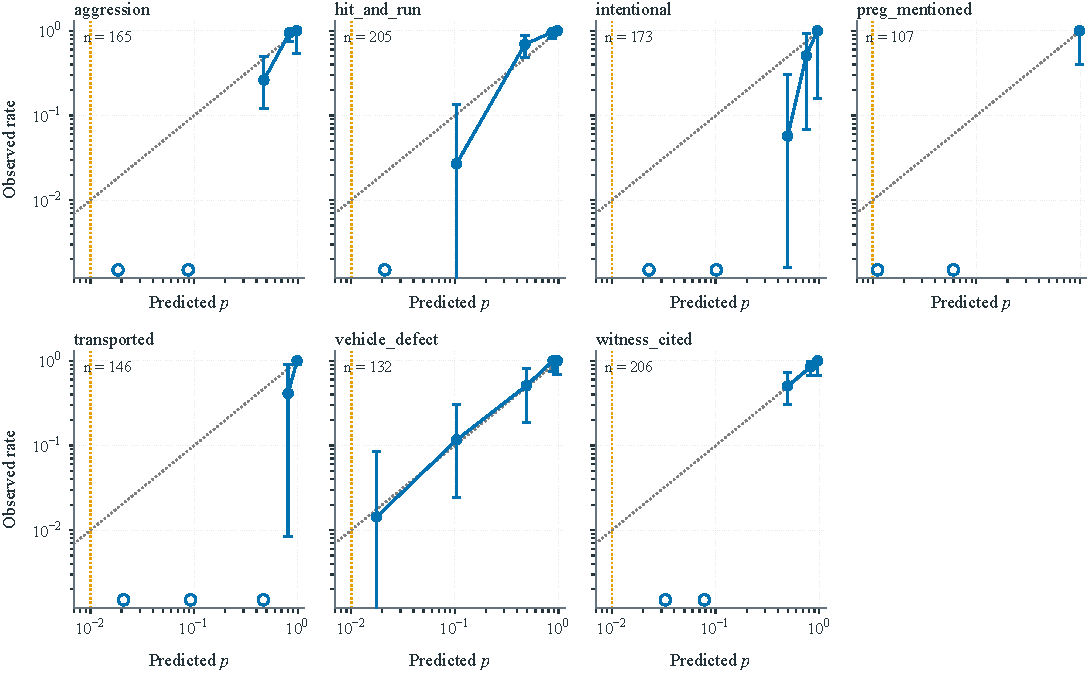
\includegraphics[width=\textwidth]{figs/FC1_gold_reliability.pdf}
\caption{Reliability against the human reference set for the seven presence variables with no
coded counterpart, which therefore do not appear in Figure~\ref{fig:calibration}. Each panel
gives the observed positive rate among the human labels within each sampling stratum,
weighted by the calibration weights of Section~\ref{sec:reference}, with approximate
intervals on the Kish effective sample size, on logarithmic axes. The dotted diagonal marks
calibration, the vertical guide the grid floor, open circles strata with no positive, and the
number of judgments is printed.}
\label{fig:goldrel}
\end{figure}

\begin{figure}[pos=!htbp]\centering
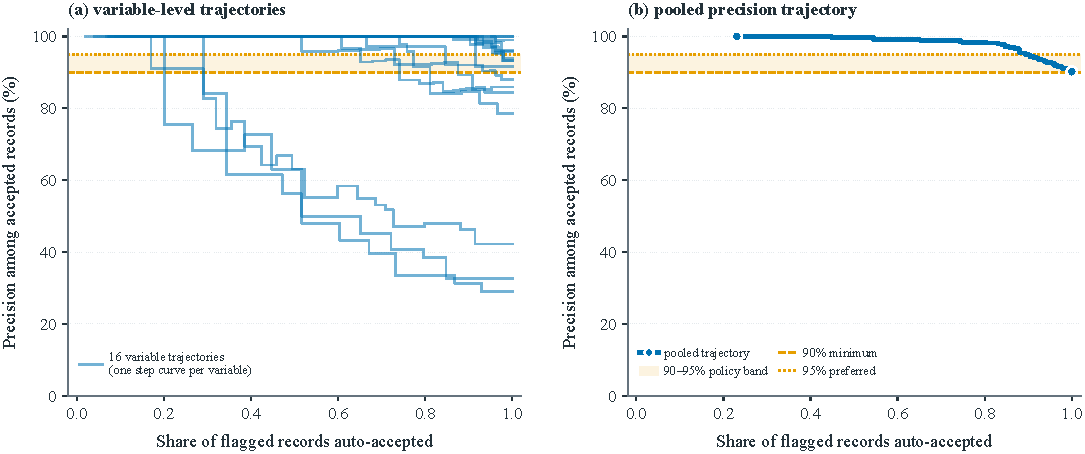
\includegraphics[width=\textwidth]{figs/FC2_gold_precision.pdf}
\caption{Precision among accepted records against the share of flagged records auto-accepted,
measured on the human reference set with the same construction as
Figure~\ref{fig:riskcoverage}b. (a) Each variable as a thin line, most holding
\PrecTargetNinety\% precision until more than four fifths of their flags are accepted.
(b) All variables pooled, crossing \PrecTargetNinetyFive\% near nine tenths of the range and
\PrecTargetNinety\% only at its right-hand end. Both panels use the whole reference set, so
they give the in-sample budgets \GoldBudgetNinetyFiveInSample\% and
\GoldBudgetNinetyInSample\%; Section~\ref{sec:res-accuracy} reports the cross-fitted budgets
\GoldBudgetNinetyFive\% and \GoldBudgetNinety\% instead.}
\label{fig:goldprec}
\end{figure}

\FloatBarrier
\section{Proofs and the implementation map}
\label{app:proofs}
\setcounter{table}{0}\setcounter{figure}{0}\setcounter{equation}{0}
\appendixtheorems

This appendix collects the mathematics on which the audit of Section~\ref{sec:evaluation}
rests. It fixes the notation shared by every statement and proves that the Murphy
decomposition of the Brier score is exact on the output grid. It then proves
Proposition~\ref{prop:floor} and Lemma~\ref{lem:noise} together with a tightness statement
for each, derives the closed form of the break-even fraction of Eq.~(\ref{eq:twostage}), and
closes with the map from every numbered equation to the released code. Every statement is written for the weighted empirical
distribution of a labeled sample, with weights $w_i$ that sum to $n$, and each holds verbatim
for the population once weighted means are replaced by expectations.

Throughout, $G \subset [0,1]$ is the finite output grid, $W_v = \sum_i w_i\,\mathbb{1}[p_i = v]$
is the weight at grid value $v$, $r_v = \frac{1}{W_v}\sum_i w_i\,\mathbb{1}[p_i = v]\,y_i$ is the
observed positive rate at $v$ whenever $W_v > 0$, $\bar{p} = \sum_v (W_v/n)\,v$ is the mean
probability, and $\bar{y} = \sum_v (W_v/n)\,r_v = \frac{1}{n}\sum_i w_i y_i$ is the base rate,
written $\rho$ in the main text. Grouping by grid value is exact rather than approximate,
because every record at a value $v$ carries the same probability. Two identities follow
directly from the definitions,
\begin{equation}
\sum_i w_i\,\mathbb{1}[p_i = v]\,(y_i - r_v) = 0 \quad\text{for every } v,\qquad
\sum_{v \in G} \frac{W_v}{n}\,(v - r_v) = \bar{p} - \bar{y}.
\label{eq:app-ident}
\end{equation}
A model is calibrated on the sample when $r_v = v$ at every grid value with $W_v > 0$, and
$w_0 = W_0/n$ denotes the weight the model places on the value zero.

\begin{lemma}[Exact Murphy decomposition on the grid]
\label{lem:murphy}
With $\mathrm{BS}$ as in Eq.~(\ref{eq:brier}) and the grouping by grid value,
\begin{equation}
\mathrm{BS} \;=\; \sum_{v \in G} \frac{W_v}{n}\,(v - r_v)^2
\;-\; \sum_{v \in G} \frac{W_v}{n}\,(r_v - \bar{y})^2 \;+\; \bar{y}\,(1 - \bar{y}),
\label{eq:app-murphy}
\end{equation}
with equality and no binning error, and the reliability term bounds the exact calibration
error of Eq.~(\ref{eq:ecegrid}) through $\mathrm{ECE}_G^2 \le \sum_v (W_v/n)(v - r_v)^2$.
\end{lemma}

\begin{pf}
Fix $v$ with $W_v > 0$. For every record at $v$,
$(v - y_i)^2 = (v - r_v)^2 + 2(v - r_v)(r_v - y_i) + (r_v - y_i)^2$. Summing with the weights
$w_i$ over the records at $v$, the middle term vanishes by the first identity of
Eq.~(\ref{eq:app-ident}). Because $y_i \in \{0, 1\}$ gives $y_i^2 = y_i$, the last term sums to
$W_v r_v - W_v r_v^2 = W_v\, r_v(1 - r_v)$. Summing over $v$ and dividing by $n$,
$\mathrm{BS} = \sum_v (W_v/n)(v - r_v)^2 + \sum_v (W_v/n)\, r_v(1 - r_v)$. Expanding
$\sum_v (W_v/n)(r_v - \bar{y})^2 = \sum_v (W_v/n)\, r_v^2 - \bar{y}^2$ and substituting gives
$\sum_v (W_v/n)\, r_v(1 - r_v) = \bar{y}(1 - \bar{y}) - \sum_v (W_v/n)(r_v - \bar{y})^2$, which
is Eq.~(\ref{eq:app-murphy}). The inequality is Jensen's inequality for the square applied to
the probability weights $W_v/n$ and the values $|v - r_v|$.
\end{pf}

\begin{proofprop}
Suppose first that the model is calibrated on the sample, so that $r_v = v$ wherever
$W_v > 0$. Then $\rho = \bar{y} = \sum_v (W_v/n)\, r_v = \sum_v (W_v/n)\, v = \bar{p}$, and
because every positive grid value is at least $\delta$,
$\bar{p} \ge \delta \sum_{v > 0} W_v/n = \delta(1 - w_0)$. Rearranging $\rho \ge \delta(1 - w_0)$
gives $w_0 \ge 1 - \rho/\delta$. The bound used only $v \ge \delta$, so it holds for every
assignment of positive grid values, and the contrapositive is the first claim. If
$\rho < \delta(1 - w_0)$, then $r_v = v$ fails at some grid value carrying weight, whatever
values the model returns. For the second claim, the second identity of Eq.~(\ref{eq:app-ident})
and the triangle inequality give
$\mathrm{ECE}_G = \sum_v (W_v/n)\,|v - r_v| \ge \bigl|\sum_v (W_v/n)(v - r_v)\bigr|
= |\bar{p} - \rho| \ge \bar{p} - \rho$. The inequality $\bar{p} \ge \delta(1 - w_0)$ holds
whether or not the model is calibrated, so $\bar{p} - \rho \ge \delta(1 - w_0) - \rho > 0$,
which is Eq.~(\ref{eq:floor}). Equality in the triangle inequality holds exactly when
$v - r_v$ has one sign at every grid value carrying weight, so $\mathrm{ECE}_G = \bar{p} - \rho$
for a model whose reliability curve lies on or above the diagonal everywhere, and the floor
$\delta(1 - w_0) - \rho$ is attained when in addition all positive weight sits at $\delta$.
Finally, let $g \colon G \to [0,1]$ be any recalibration map. If $g(p)$ is calibrated then
$\sum_v (W_v/n)\, g(v) = \rho < \delta(1 - w_0)$, so $g$ must send some positive grid value
carrying weight below $\delta$. The maps of Eq.~(\ref{eq:platt}) can do so and the model
cannot, which is why the floor is a property of the grid and not of the ranking.
\end{proofprop}

\begin{prooflem}
Write the coded field as $y' = y\,(1 - m)$, where $m$ is an omission indicator with
$\Pr(m = 1 \mid y = 1, p = v) = f_v$, so that $y' = 1$ implies $y = 1$ and
$r'_v = \Pr(y' = 1 \mid p = v) = (1 - f_v)\, r_v$. The weights $W_v$ depend on $p$ alone and are
therefore the same under both references. Since $0 \le f_v \le 1$, $r'_v \le r_v$, which is
the first claim. If $(1 - f_v)\, r_v \ge v$ then $v \le r'_v \le r_v$, so
$|v - r'_v| = r'_v - v \le r_v - v = |v - r_v|$, which is the second claim, and summing with the
weights $W_v/n$ over every grid value with $W_v > 0$ gives Eq.~(\ref{eq:noise}). Under that
condition the gap is exact rather than an inequality,
\begin{equation}
\mathrm{ECE}_G(y) - \mathrm{ECE}_G(y') \;=\; \sum_{v \in G} \frac{W_v}{n}\,(r_v - r'_v)
\;=\; \sum_{v \in G} \frac{W_v}{n}\, f_v\, r_v \;=\; \Pr(y = 1,\; y' = 0),
\label{eq:app-gap}
\end{equation}
the share of records that the narrative reference marks positive and the coded field does
not, which is the narrative-only cell measured in Section~\ref{sec:res-frontier}. Where the
condition fails at some $v$, $r'_v < v$ and $|v - r'_v| = v - r'_v$. This exceeds $|v - r_v|$
whenever $r_v < v$, and whenever $r_v \ge v$ with $2v > r_v + r'_v$, so omission then inflates
the measured error and the bias reverses on that part of the grid. If the coded field also
records factors the narrative does not state, $r'_v$ can exceed $r_v$ and the direction of the
bias is no longer determined by the omission rate alone.
\end{prooflem}

\begin{lemma}[Break-even fraction]
\label{lem:breakeven}
Under the cost model of Eq.~(\ref{eq:cost}) with $k_f > k_s$, the break-even fraction of
Eq.~(\ref{eq:twostage}) has the closed form
\begin{equation}
q^{*} \;=\; \frac{\beta\,(k_f - k_s)}{\alpha + \beta k_f + b\bar{\ell}},\qquad
\frac{\partial q^{*}}{\partial \bar{\ell}} \;=\; -\,\frac{b\,\beta\,(k_f - k_s)}{(\alpha + \beta k_f + b\bar{\ell})^2},\qquad
\frac{\partial \ln q^{*}}{\partial \ln \bar{\ell}} \;=\; -\,\frac{b\bar{\ell}}{\alpha + \beta k_f + b\bar{\ell}},
\label{eq:app-breakeven}
\end{equation}
so $q^{*}$ decreases in narrative length, and its elasticity with respect to length equals
minus the share of the full-schema token count that the text contributes.
\end{lemma}

\begin{pf}
Screening costs less than coding everything once exactly when
$T(k_s, \bar{\ell}) + q\,T(k_f, \bar{\ell}) < T(k_f, \bar{\ell})$, that is when
$q < 1 - T(k_s, \bar{\ell})/T(k_f, \bar{\ell}) = [T(k_f, \bar{\ell}) - T(k_s, \bar{\ell})]/T(k_f, \bar{\ell})$.
The intercept $\alpha$ and the text term $b\bar{\ell}$ cancel in the difference, which leaves
$\beta(k_f - k_s)$ in the numerator. Differentiating the quotient in $\bar{\ell}$ gives the
second expression, and multiplying it by $\bar{\ell}/q^{*}$ gives the third. When
$\beta k_f$ dominates $b\bar{\ell}$ the elasticity is small, which is the claim of
Section~\ref{sec:schema} that the schema rather than the text governs the two-stage design.
\end{pf}

The weighting of Eq.~(\ref{eq:ht}) is a calibration estimator rather than an inverse-probability
one, and the distinction matters for what can be claimed about it. The classical result is that
$\mathbb{E}\bigl[\sum_{i \in s} z_i/\pi_i\bigr] = \sum_{i \in U} z_i$ for any sample $s$ drawn
from the frame $U$ with inclusion probabilities $\pi_i > 0$, because
$\mathbb{E}\,\mathbb{1}[i \in s] = \pi_i$ \citep{horvitz1952generalization}. That result is
background here rather than an assertion about this reference set, because the greedy draw and
the identifier screen of Section~\ref{sec:reference} leave no $\pi_i$ that can be written down.
The weights used instead satisfy the calibration equations exactly, so the weighted count of
every cell reproduces its population count, and the resulting estimator is design-consistent
under the condition that labeling is uninformative about the outcome within a cell
\citep{deville1992calibration}. The ratio of two weighted sums is consistent but not unbiased,
with a bias of order $1/n$ \citep{sarndal1992model}, which is why the percentile interval of
Eq.~(\ref{eq:htvar}) is re-centered by the bootstrap estimate of that bias. Table~\ref{tab:eqmap} lists, for every numbered equation of
Section~\ref{sec:methods}, the released script, the function and the result file that compute
it, so that a reader can locate the implementation of each quantity without searching the
repository.

\begin{sidewaystable}[!htbp]
\centering
\rmfamily\small
\setlength{\tabcolsep}{3.0pt}
\jevrotcaption{tab:eqmap}{Where each formalized quantity is computed.}
\begin{threeparttable}
\begin{tabular}{>{\raggedright\arraybackslash}p{64.1pt}>{\raggedright\arraybackslash}p{132.5pt}>{\raggedright\arraybackslash}p{135.4pt}>{\raggedright\arraybackslash}p{130.6pt}>{\raggedright\arraybackslash}p{136.7pt}}
\toprule
\jevheadp{equation} & \jevheadp{quantity} & \jevheadp{script (\texttt{src/})} & \jevheadp{function} & \jevheadp{result file (\texttt{data/})} \\
\midrule
Eq.~(\ref{eq:gate}) & gating operator and no-match override & \texttt{s06\_flatten.py} & \texttt{flatten} & \texttt{stage2\_flat.parquet} \\
Eq.~(\ref{eq:leak}) & leakage rate $\lambda_v$ & \texttt{s06\_flatten.py} & \texttt{flatten} & \texttt{stage2\_leakage.json} \\
Eq.~(\ref{eq:ht}) & H\'ajek ratio with calibration weights $w_i$ & \texttt{s05b\_design\_weights.py; s17\_gold\_analysis.py} & \texttt{design\_weights; wrate, block} & \texttt{gold\_design\_weights.csv; gold\_analysis.json} \\
Eq.~(\ref{eq:htvar}) & stratified cluster bootstrap interval & \texttt{s07\_metrics.py} & \texttt{cluster\_bootstrap; weighted\_bootstrap} & \texttt{analysis.json; gold\_analysis.json} \\
Eq.~(\ref{eq:brier}) & Brier score and Murphy decomposition & \texttt{s07\_metrics.py} & \texttt{brier, brier\_decomposition} & \texttt{analysis.json} \\
Eq.~(\ref{eq:ece}) & expected and maximum calibration error, equal-mass bins & \texttt{s07\_metrics.py} & \texttt{ece, mce, equal\_mass\_bins} & \texttt{analysis.json} \\
Eq.~(\ref{eq:ecegrid}) & exact calibration error on the output grid & \texttt{s07\_metrics.py} & \texttt{ece\_discrete, discrete\_reliability} & \texttt{analysis.json; gold\_analysis.json} \\
Eq.~(\ref{eq:cox}) & calibration slope and intercept & \texttt{s07\_metrics.py} & \texttt{calibration\_slope} & \texttt{analysis.json; gold\_analysis.json} \\
Eq.~(\ref{eq:spieg}) & Spiegelhalter statistic & \texttt{s07\_metrics.py} & \texttt{spiegelhalter\_z} & \texttt{analysis.json; gold\_analysis.json} \\
Eq.~(\ref{eq:floor}) & resolution-floor bound & \texttt{s07\_metrics.py} & \texttt{resolution\_floor\_report} & \texttt{analysis.json} \\
Eq.~(\ref{eq:prec}) & precision and coverage over flagged records & \texttt{s07\_metrics.py} & \texttt{precision\_coverage, coverage\_at\_precision} & \texttt{analysis.json} \\
Eq.~(\ref{eq:budget}) & review budget $H(\pi^*)$, cross-fitted & \texttt{s07\_metrics.py; s17\_gold\_analysis.py} & \texttt{positive\_review\_budget; held\_out\_budget} & \texttt{analysis.json; gold\_analysis.json} \\
Eq.~(\ref{eq:riskcov}) & risk--coverage curve and area & \texttt{s07\_metrics.py} & \texttt{risk\_coverage, aurc, coverage\_at\_risk} & \texttt{analysis.json} \\
Eq.~(\ref{eq:noise}) & one-sided reference-noise bound & \texttt{s17\_gold\_analysis.py} & \texttt{narrative\_only} & \texttt{gold\_analysis.json} \\
Eq.~(\ref{eq:cost}) & token cost model & \texttt{s08\_cost\_model.py} & \texttt{main} & \texttt{cost\_model.json} \\
Eq.~(\ref{eq:twostage}) & two-stage cost and break-even fraction & \texttt{s08\_cost\_model.py; pricing.py} & \texttt{main; jev\_cost\_per\_1k} & \texttt{cost\_model.json} \\
Eq.~(\ref{eq:platt}) & Platt and isotonic recalibration, split over narratives & \texttt{s17\_gold\_analysis.py} & \texttt{recalibration} & \texttt{gold\_analysis.json} \\
Eq.~(\ref{eq:kappa}) & Cohen's kappa, weighted against the reference set & \texttt{s07\_metrics.py; s16\_gold\_ingest.py} & \texttt{cohen\_kappa} & \texttt{gold\_reliability.json; gold\_analysis.json} \\
Eq.~(\ref{eq:cp}) & Clopper--Pearson interval & \texttt{s07\_metrics.py} & \texttt{clopper\_pearson} & \texttt{analysis.json} \\
Eq.~(\ref{eq:mcnemar}) & McNemar test & \texttt{s07\_metrics.py} & \texttt{mcnemar} & \texttt{analysis.json} \\
\bottomrule
\end{tabular}
% \begin{tablenotes}[flushleft]\small\rmfamily
% \item \textit{Note:}~Scripts are in \texttt{paper1/src/} and result files in \texttt{paper1/data/} of the released repository. Every equation in Section~\ref{sec:methods} maps to a function that a reader can execute on the released outputs.
% \end{tablenotes}
\end{threeparttable}
\end{sidewaystable}

